\section{Analysis}

\subsection{Description of the simulation}
We consider a set of Monte Carlo cluster simulations, developed with the Monte Carlo
code MOCCA of Hypki et al. 2013 (see also Giersz et al. 1998). The simulations
include an initial mass function, stellar evolution, primordial binaries, and a
relatively high number of particles, providing a realistic description of the
long-term evolution of \acp{GC} with a single stellar population.

All the simulation had a metallicity of [Fe/H]=$-$1.3 and a Kroupa (2001) initial
mass function. The first simulation (from Giersz et al. 2015, kindly shared by the
authors) contain an \ac{IMBH} of $10^4$ M$_\odot$ and its initial condition is drawn from a
King model with concentration parameter W$_0 $=6, 6.9$\cdot10^5$ initial number of particles,
95\% of which are binary systems. We consider two snapshots of the simulation on at
10 and one at 7 Gyr. We call these snapshots SIM1-IMBH and SIM2-IMBH, respectively.
Other two simulations (from Downing et al. 2010, kindly shared by the authors), do
not contain an \ac{IMBH} and have an initial number of particles of 5$\cdot10^5$ and 2$\cdot10^6$, 10\%
of initial binaries, and initial conditions drawn from a Plummer (1911) model with a
ratio between the initial tidal radius and half-mass radius of 75. We consider a 11
Gyr snapshot for both simulations and we call them SIM3-NOIMBH and SIM4-NOIMBH,
respectively.

We summarize in Table \ref{tab:overview_simulation} the properties of the simulations for the time-snapshots
considered. 


\begin{table}[htbp]
\centering
\begin{tabular}{ c | c | c | c | c | c }
\makecell{Name of the \\simulation} & \makecell{Number of \\ particles} & Total mass [M\(_\odot\)]& \makecell{Mass of the \\ \ac{IMBH} [M\(_\odot\)]}& r\(_\mathrm{m}\) [pc] & Age [Gyr]\\
\hline			
  SIM 1 - IMBH & 1026735 & 3.09\(\cdot 10^5\) & 10102 & 4.13 & 10\\
  SIM 2 - IMBH & 1079376& 3.26\(\cdot 10^5\) & 8902.3 & 3.58 & 7\\
  SIM 3 - NOIMBH & 468627& 1.73\(\cdot 10^5\)& 0 & 7.89 & 11\\
  SIM 4 - NOIMBH & 1851556& 6.70\(\cdot 10^5\)& 0 & 5.41 & 11\\

\end{tabular}
\caption{Overview of the data of the simulations. We show the basic properties of each simulation which are numper of particles, the total mass, the mass of the \ac{IMBH}, the half mass radius and the age. The half mass radius is defined by the radius which includes half of the mass of the whole system.}
\label{tab:overview_simulation}
\end{table}

The output of the simulations relevant for our work are for each star: the position
vector x, the velocity vector v in Cartesian and polar coordinates, mass, luminosity, magnitude b and v band and whether
the star is a binary or not.
\\
To get familiar with the simulation we first have a look at the distribution of the star positions.
\begin{figure}[htbp] 
\centering
\begin{subfigure}{0.9\textwidth}
	\centering
  	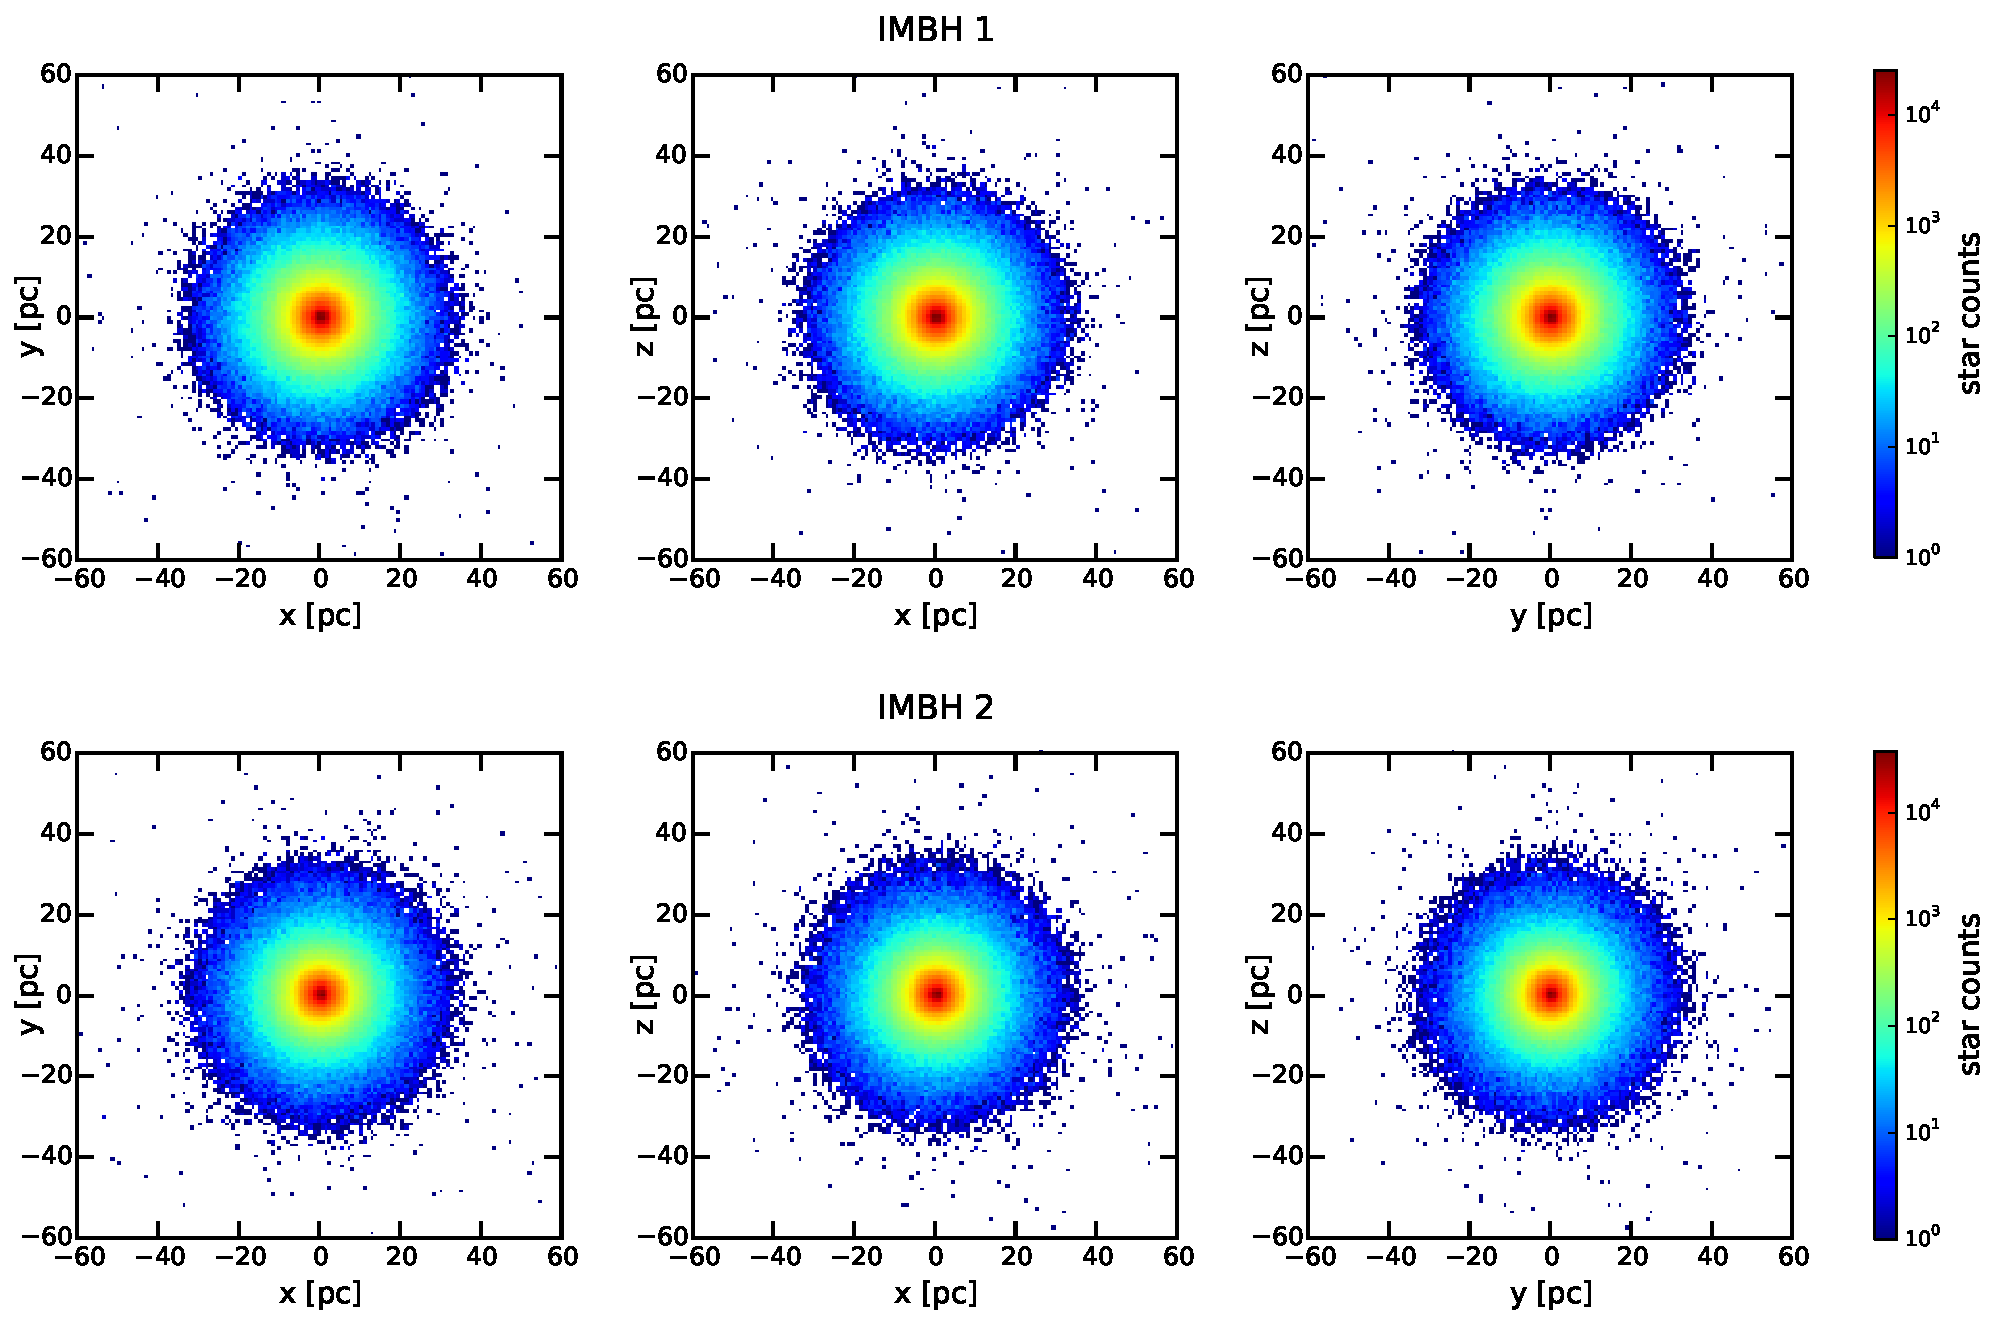
\includegraphics[width=\textwidth]{Plots/position_scatter_plot_IMBH.pdf}
  	\caption{SIM 1 \& SIM 2. The \acp{GC} are spread until 100 pc with most of the stars located in the inner 40 pc.}
 	\label{fig:pos_scat_IMBH}
\end{subfigure}
\\
\begin{subfigure}{0.9\textwidth}
	\centering
  	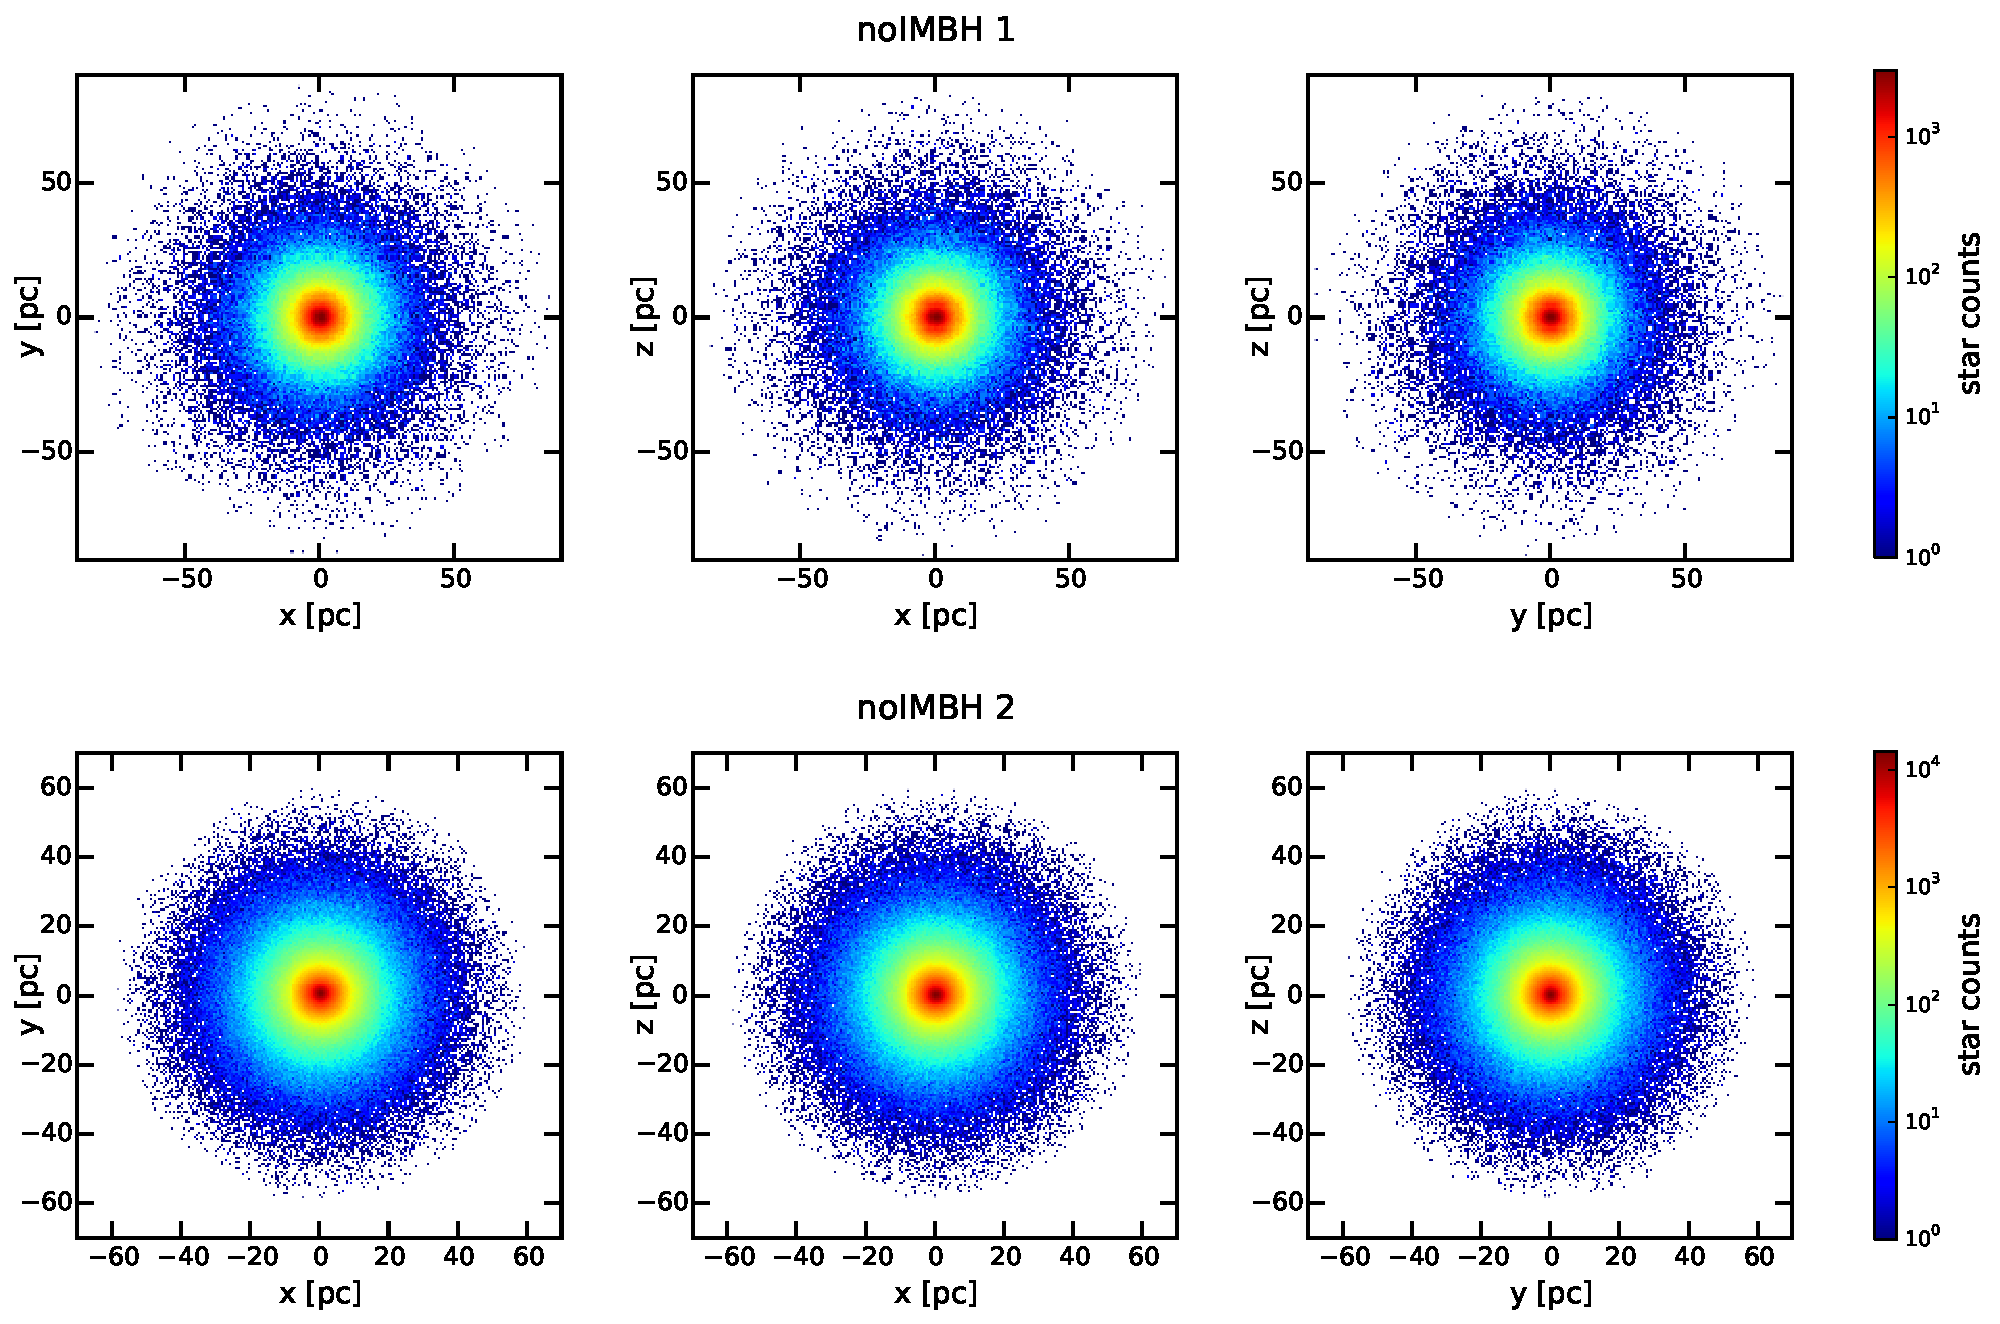
\includegraphics[width=\textwidth]{Plots/position_scatter_plot_noIMBH.pdf}
  	\caption{SIM 3 \& SIM 4. The \ac{GC} is spread until 90 pc (SIM3) and until 60 pc (SIM4).}
 	\label{fig:pos_scat_noIMBH}
\end{subfigure}

\caption{Spatial distribution of stars in the simulated \acp{GC}. The stars are distributed spherically with most of the stars in the inner part. The stars of the \acp{GC} with \ac{IMBH} are less spread in the outer parts except very few which are far outside. This is simply due to the different initial concentration conditions of the simulations. In the \acp{GC} without \ac{IMBH} the stars in the outer part are less accumulated but the furthermost stars still in the main sphere.}
\label{fig:position_scatter}
\end{figure}

\begin{figure}[htbp] 
\centering
	\begin{subfigure}{0.9\textwidth}
		\centering
	  	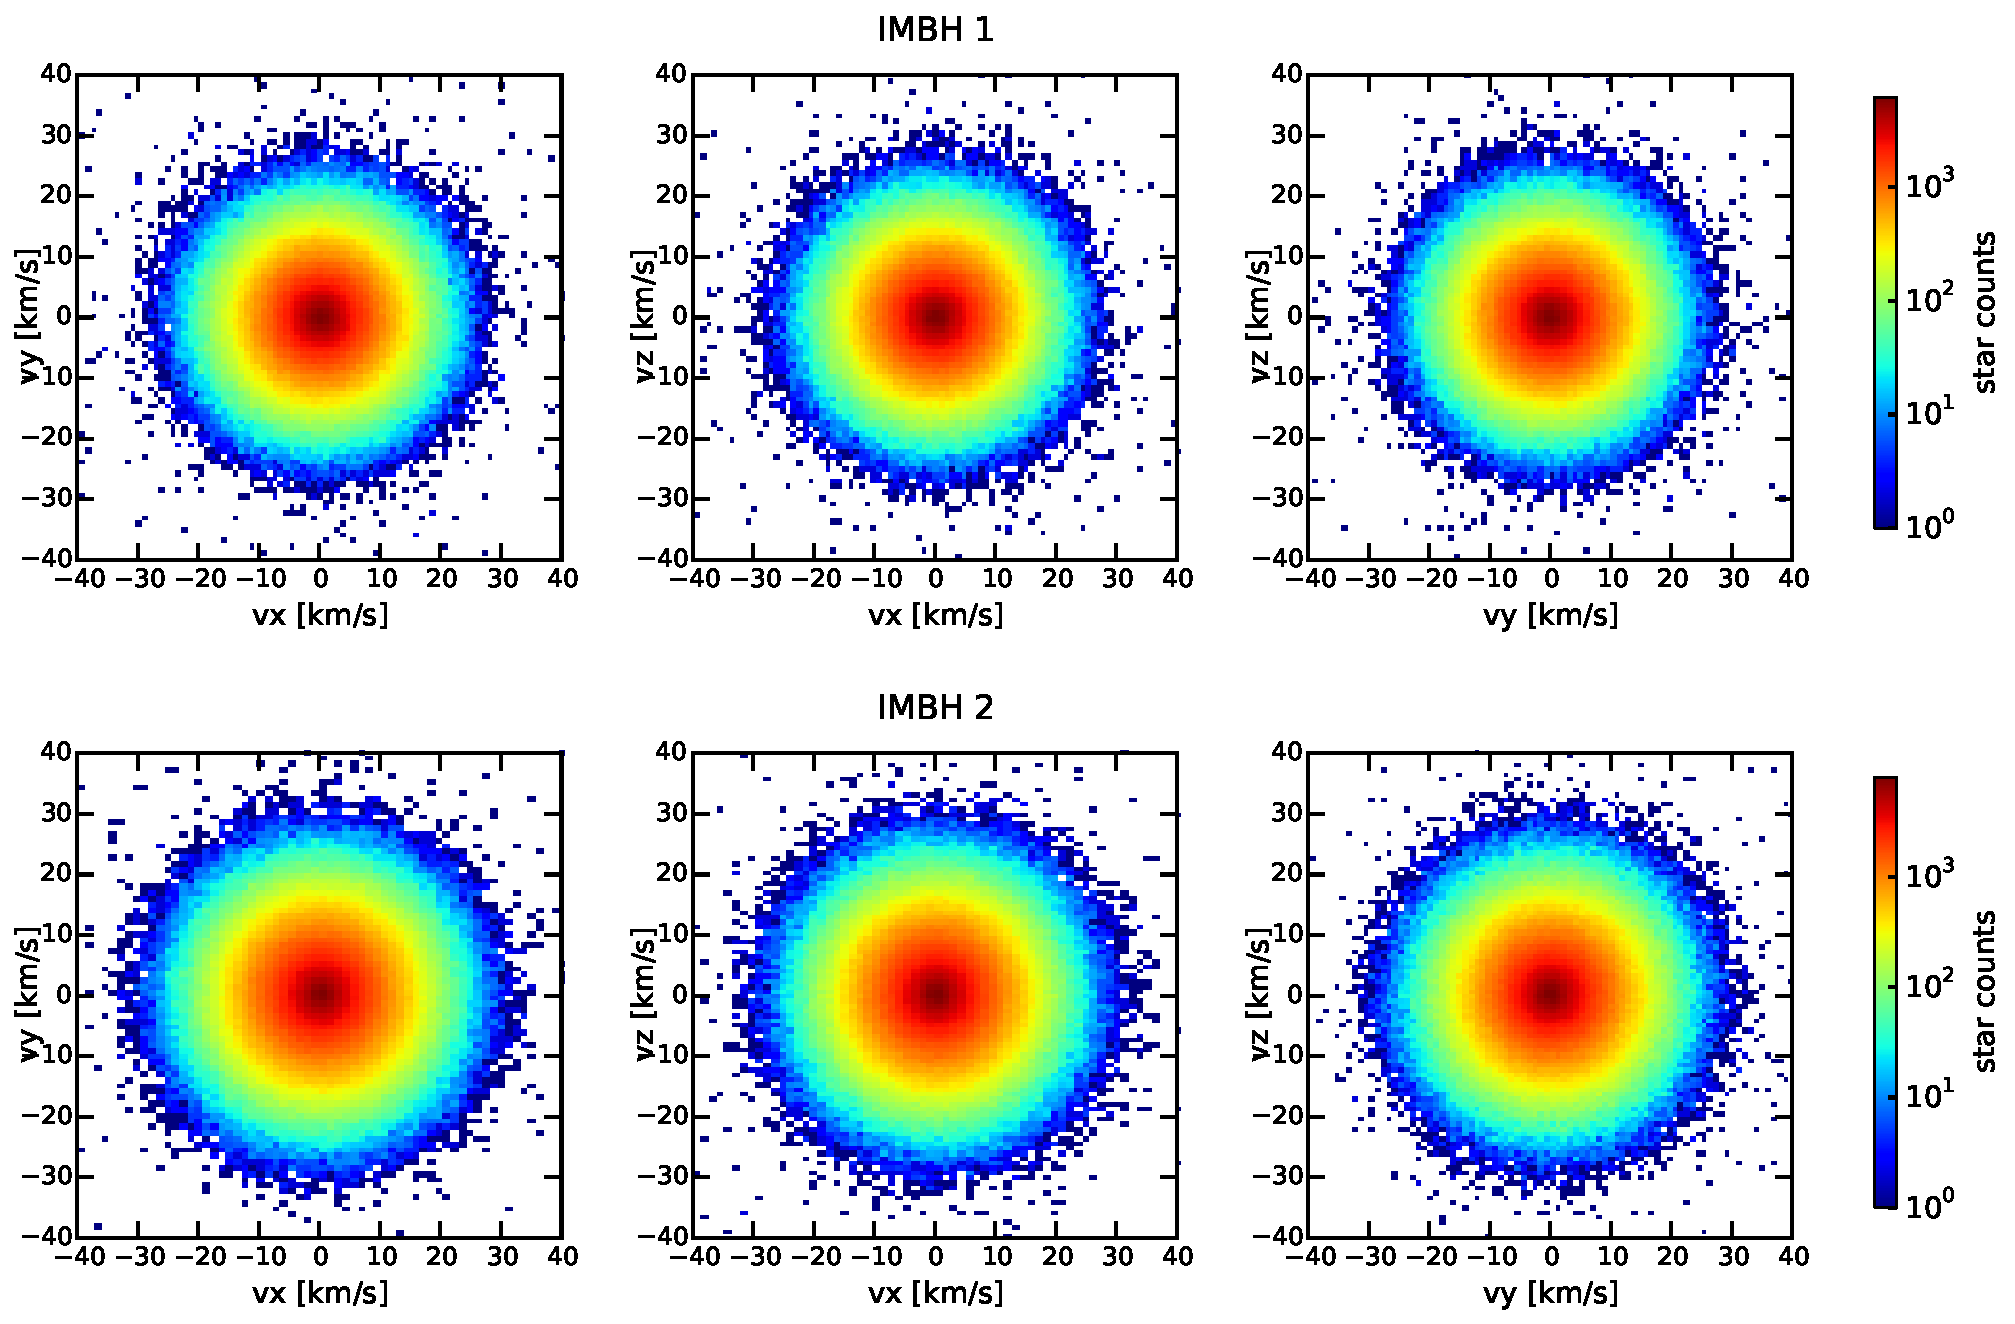
\includegraphics[width=\textwidth]{Plots/velocity_scatter_IMBH.pdf}
	  	\caption{SIM 1 \& SIM 2. The stars' velocities are spread until 120 km/s with most of them reaching 30 km/s.}
	 	\label{fig:vel_scat_IMBH}
	\end{subfigure}
	\\
	\begin{subfigure}{0.9\textwidth}
		\centering
	  	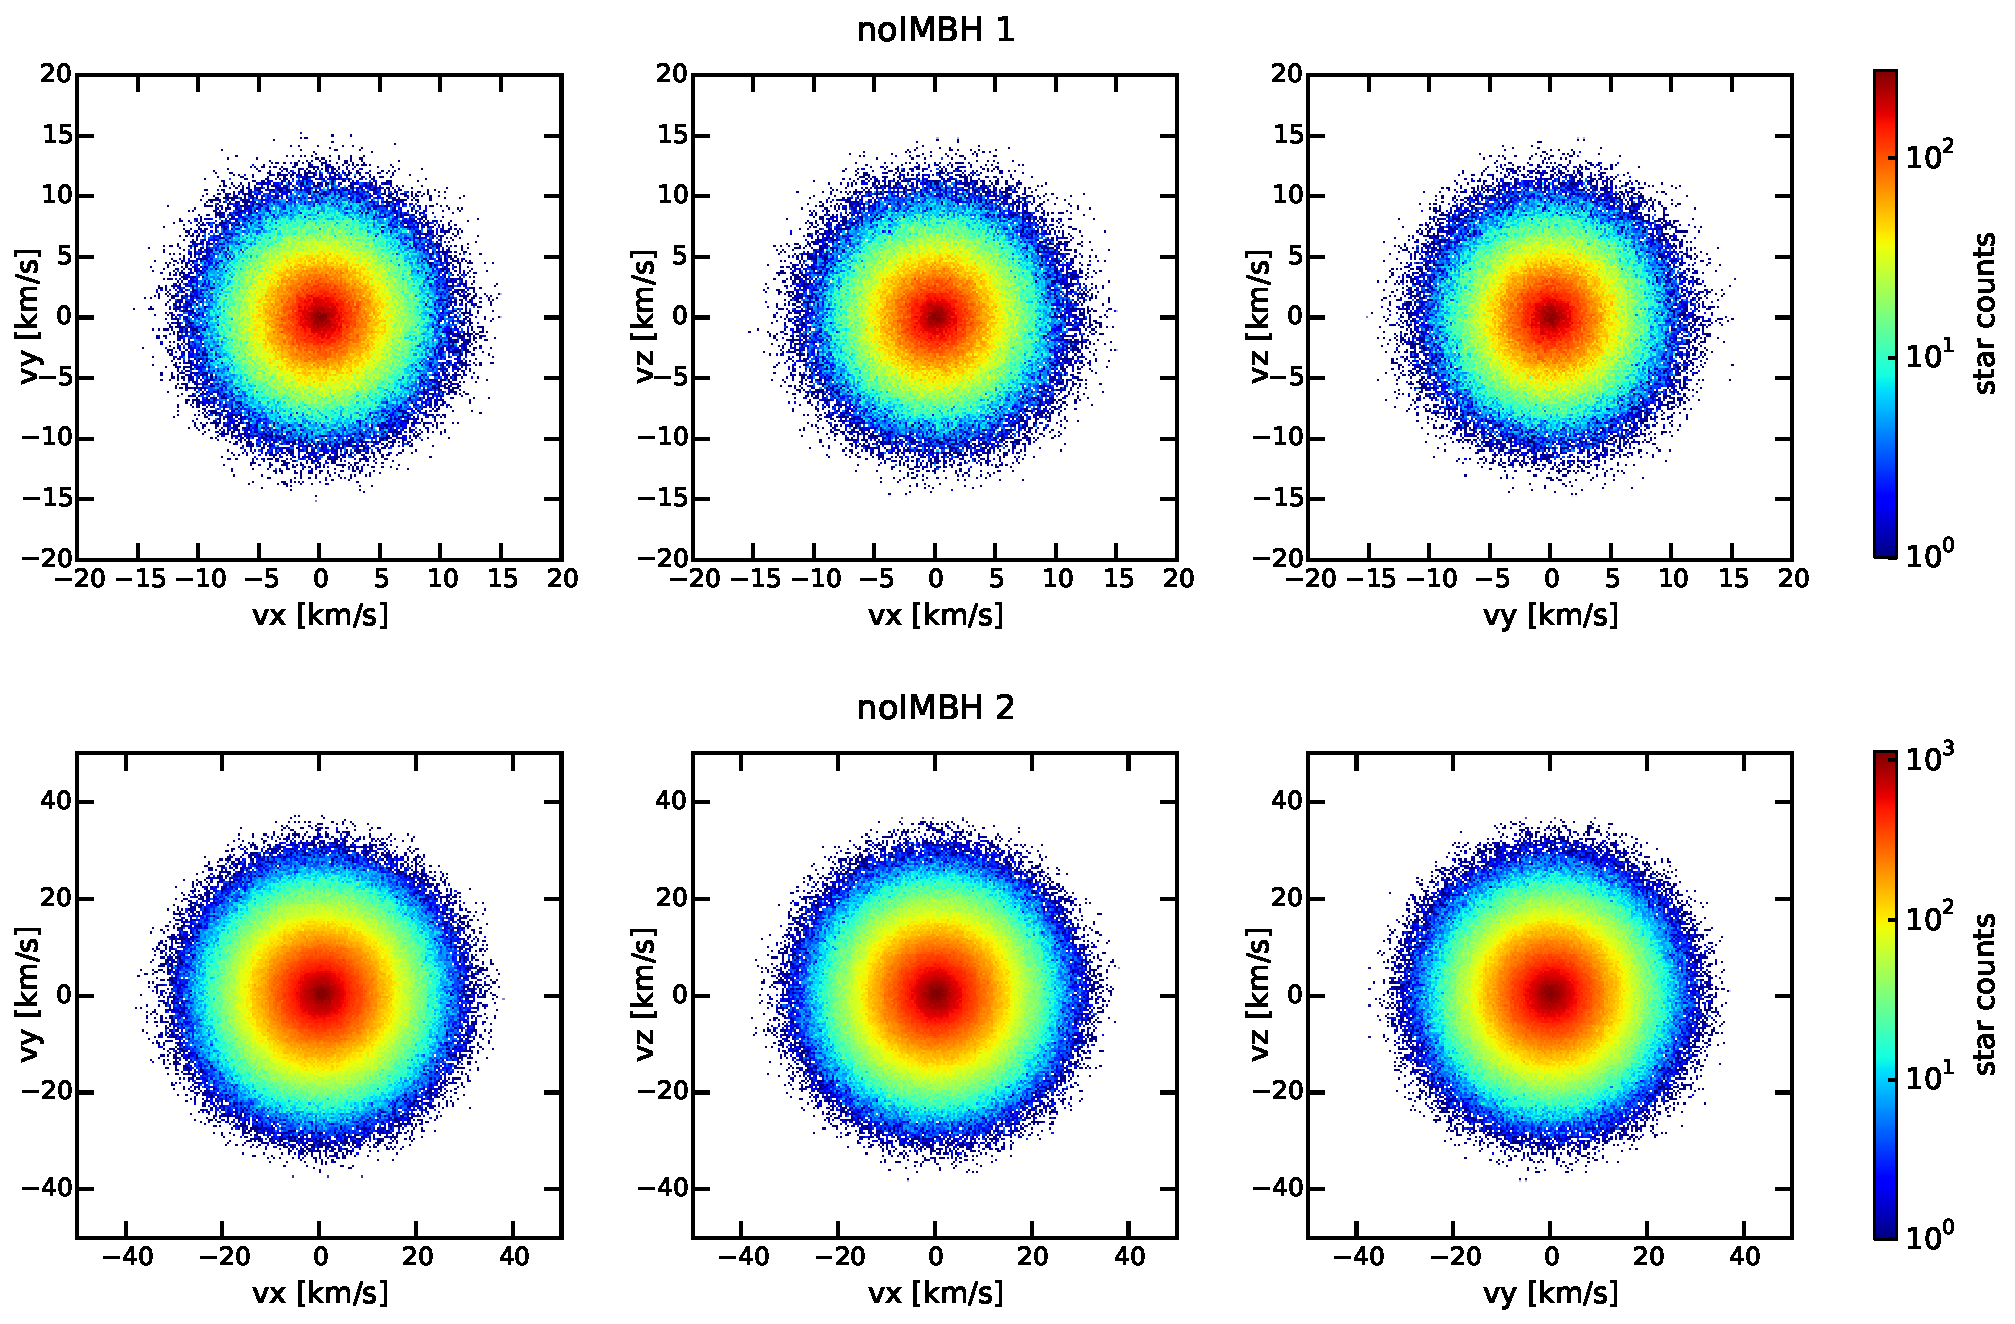
\includegraphics[width=\textwidth]{Plots/velocity_scatter_noIMBH.pdf}
	  	\caption{SIM 3 \& SIM 4. The stars' velocities are spread until 15 km/s for SIM 3 whereas they spread until 40 km/s for SIM 4.}
	 	\label{fig:vel_scat_noIMBH}
	\end{subfigure}

\caption{Velocity distribution of stars in the simulated \acp{GC}. The velocities are isotropically spread around \(\vec{v}=0\). Most of the stars have low or no velocity while a few have high velocities in different directions. There are no overall streaming motions.}
\label{fig:velocity_scatter}
\end{figure}


\subsection{Investigation in color magnitude space}
As mentioned in \ref{cmd_theory} the \ac{CMD} is showing a star's evolution stage dependend on its position. If one do not know age or metallicity of the system isochrones can be fitted on the \ac{CMD}. We plot several isochrones (see section \ref{cmd_theory}) to our \ac{CMD} to determine which one fits best. This will give us the age and the metallicity of the system. 
\begin{figure}[htbp]
\centering
\includegraphics[width=0.7\textwidth]{Plots/cmd_isochrones}
\caption{Color magnitude diagram of SIM 1 overplotted with different isochrones. We recognize how we can determine the age based on the turn off point. This verifies the age and the metallicity of this \ac{GC} of 10 Gyr and 0.001.}
	\label{fig:cmd_isochrones}
\end{figure}



\subsection{Investigation in phase space}

First we will investigate the \ac{GC} in phase space for the set of simulations that we will use throughout this work. We will start with the velocity dispersion and the anisotropy parameter then we will have a density profile and from that get the potential. 

\subsubsection{Kinematics}
With equation \eqref{eq:vel_disp} from section \ref{kin_prof_theory} we can calculate the velocity dispersion in each coordinate direction \(\sigma_\mathrm{r},\sigma_\theta,\sigma_\phi\). For every bin we take the same amount of stars and calculate the dispersion along the radius of the \ac{GC}. As radial values we use the average radius of the stars falling in the bins. To compare all simulations we plot the dispersion over the half-mass radius. The half mass radii of the simulations can be taken from table \ref{tab:overview_simulation}. 
\begin{figure*}[htbp]
	\centering
	\begin{subfigure}{0.475\textwidth}
		\centering
		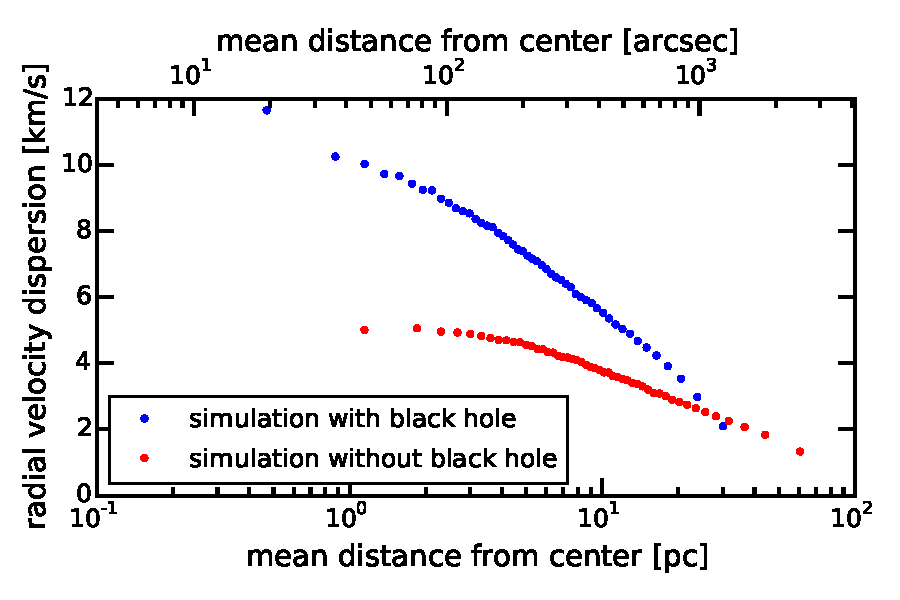
\includegraphics[width=\textwidth]{Plots/radial_velocity_dispersion.pdf}
		\caption{Radial velocity dispersions}
		\label{[fig:radial_vel_disp]}
	\end{subfigure}
	\hfill
	\begin{subfigure}{0.475\textwidth}
		\centering
		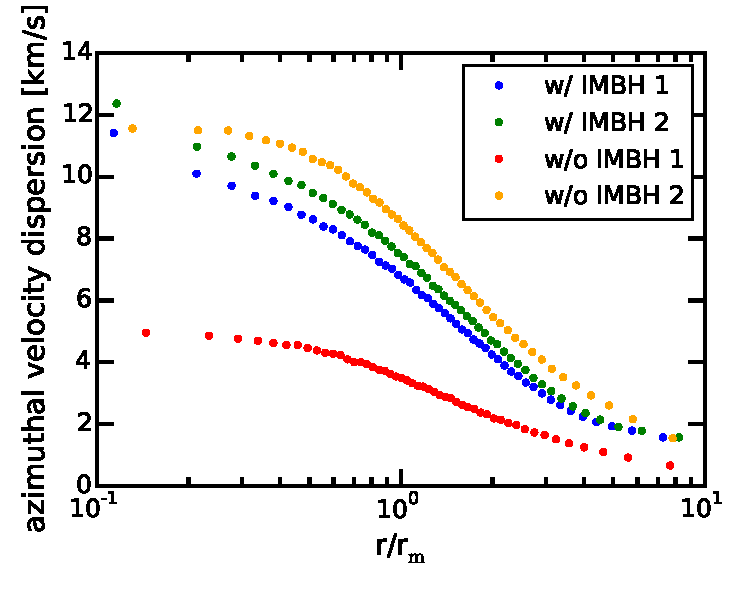
\includegraphics[width=\textwidth]{Plots/azimuthal_velocity_dispersion.pdf}
		\caption{Azimuthal velocity dispersions}
		\label{[fig:azimuthal_vel_disp]}
	\end{subfigure}
	\vskip\baselineskip
	\begin{subfigure}{0.475\textwidth}
		\centering
		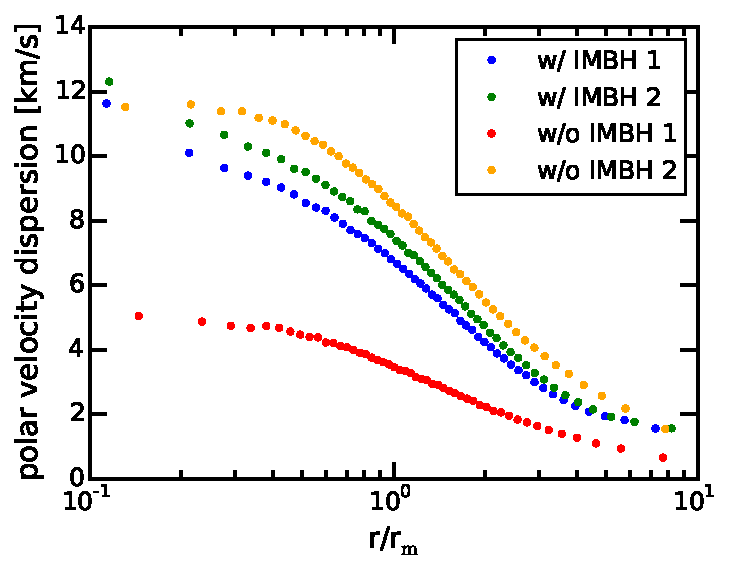
\includegraphics[width=\textwidth]{Plots/polar_velocity_dispersion.pdf}
		\caption{Polar velocity dispersions}
		\label{[fig:polar_vel_disp]}
	\end{subfigure}


	\caption{Velocity dispersion profiles as a function of the radius in units of the effective radius \(\mathrm{r_{eff}}\). They are binned in a way that each bin contains the same amount of stars. We can see that the velocity dispersion of the simulation with \ac{IMBH} rises towards the centre whereas the simulation without \ac{IMBH} exhibits a cored profile.}
\end{figure*}
As expected there is a rise in the centre for the simulations with \ac{IMBH}. This is due the high gravitational potential of the \acp{IMBH} which disturbs the dynamics of close stars. 



\par Anisotropy can be calculated from equation \eqref{eq:anisotropy} in \ref{kin_prof_theory}. It is binned the same way as the velocity dispersions and given in units of the half-mass radius.
\begin{figure}[htbp]
	\centering
	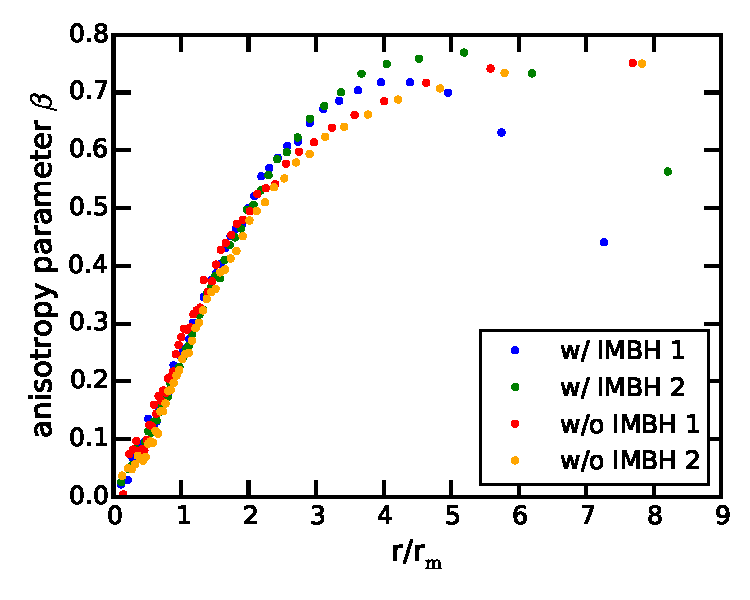
\includegraphics[width=0.475\textwidth]{Plots/anisotropy_parameter_beta.pdf}
	\caption{Anisotropy parameter \(\beta\). All simulations show isotropy in the centre and radial anisotropy in the intermediate regions. The simulations with \acp{IMBH} have a peak at 4 and 5 effective radii where they are most radial anisotropic. Some difference in anisotropy is observable between the simulations with and without \ac{IMBH}. This is due to different truncation prescriptions used in the simulations. We note that within \(\approx 2\mathrm{r_m}\) all simulations exhibit the same anisotropy profile.}
	\label{fig:anisotropy_param}
\end{figure}
In the central \(\approx 2\mathrm{r_m}\) of all \acp{GC} there is nearly the same anisotropy:isotropy in the centre \& radial anisotropy while going in the outer parts. That means the systems are radial anisotropic. The \acp{GC} with \ac{IMBH} are most radially anisotropic at about 4 effective radii. The other \acp{GC} are becoming more radial anisotropic the further away from the centre it is. The difference is due to different truncation prescriptions of the simulation.

\subsubsection{Spatial distribution}
The density profile shows the density calculated by equation \eqref{eq:density} of the system over its radius. As bins we use radial shells with logarithmic spacing chosen so that they are at least 100 stars per bin to have a reliable statistic. Outside of the cluster the density is set to 0. In the centre of the \acp{GC} (the distance of the 300th star of each simulation) we extrapolate the density profiles by setting it to the constant value of the innermost shell. 

\begin{figure}[htbp]
	\centering
	\begin{subfigure}{0.475\textwidth}
		\centering
		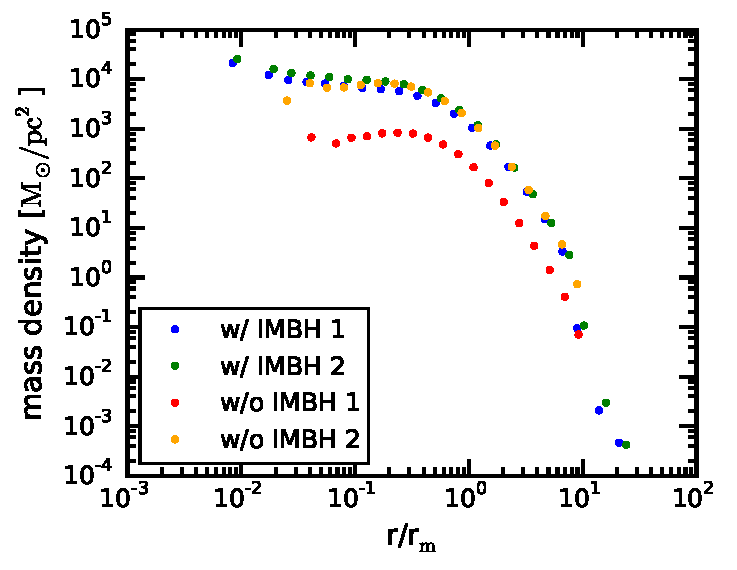
\includegraphics[width=\textwidth]{Plots/density_profiles.pdf}
		\caption{Mass density profiles of all four simulations.}
		\label{fig:mass_dens_points}
	\end{subfigure}
	\hfill
	\begin{subfigure}{0.475\textwidth}
		\centering
		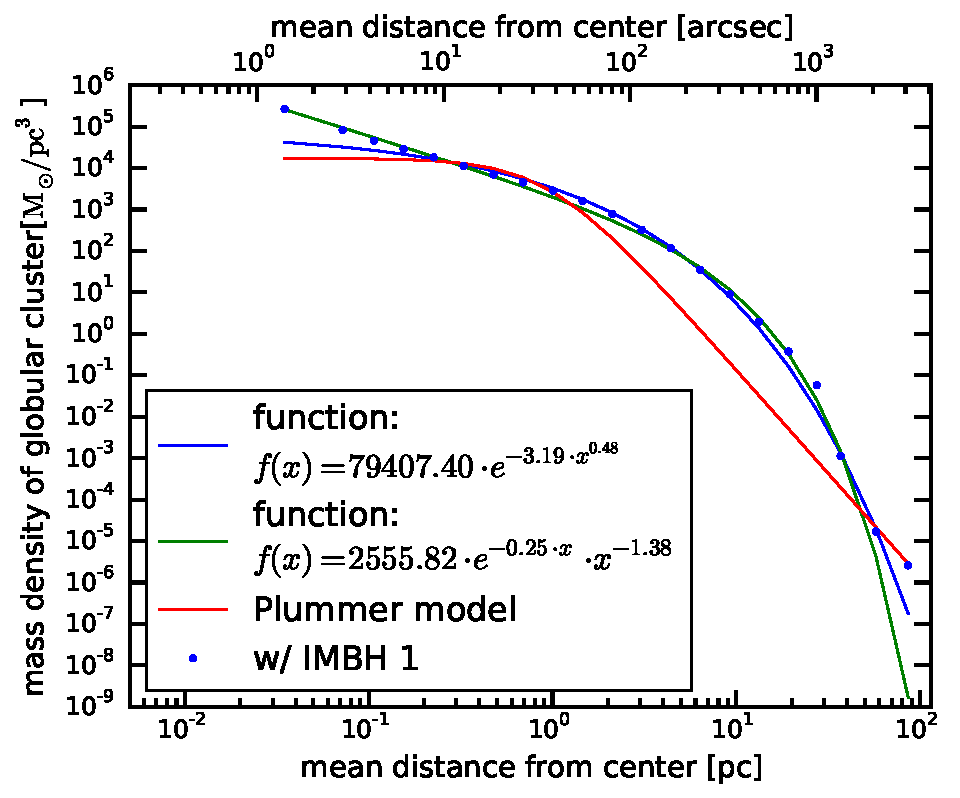
\includegraphics[width=\textwidth]{Plots/density_prof_analytic.pdf}
		\caption{Analytically fitted mass density profile of SIM 1.}
		\label{fig:mass_dens_ana}
	\end{subfigure}
	\vskip\baselineskip
	\begin{subfigure}{0.475\textwidth}
		\centering
		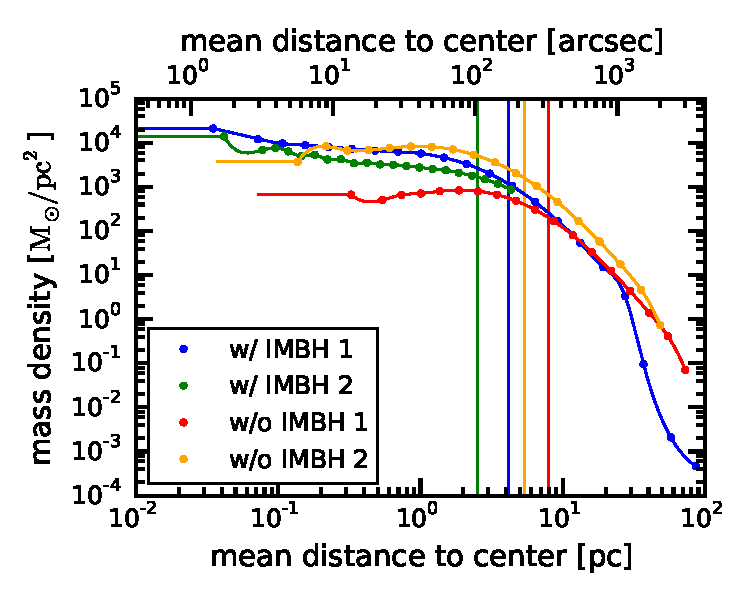
\includegraphics[width=\textwidth]{Plots/density_profiles_interpolated.pdf}
		\caption{Interpolated mass density profiles of SIM 1 and SIM 3.}
		\label{fig:mass_dens_intpol}
	\end{subfigure}
	\caption{Mass density profiles. The density in \(\frac{M_{\odot}}{pc^2}\) is plotted against the effective radius. The density of the \ac{GC} with \ac{IMBH} is everywhere larger than the density of the \ac{GC} without \ac{IMBH}. In the centre there is a raise in the density of the \ac{GC} with \ac{IMBH} whereas the other \ac{GC} stays approximately on the same level. Both start decreasing at about 0.5 \(\mathrm{r_eff}\). We can see in Panel \ref{fig:mass_dens_intpol} that it is not simple to find an analytical function describing the density globally for both low \& high radius. That is why we interpolate it in Panel \ref{fig:mass_dens_intpol}. Everything out of the \ac{GC} is set to 0 while the innermost density is set to be the value of the innermost point.}
	\label{fig:mass_density_profile}
\end{figure}
We try to find a analytic fitting function to the density profile for SIM 1 to calculate the potential from the Poisson's equation \eqref{eq:Poisson}. We use two variations of an exponential function which could fit well. Also we want to check if the density follows a classical \ac{GC} profile which i.e. is the Plummer profile. In Figure \ref{fig:mass_dens_ana} we see that we can not find a simple fitting function nor a classical profile which describes the density. To get a analytical function we continue by using the interpolated density given in Figure \ref{fig:mass_dens_intpol}.

\par As we said in section \ref{sec2.1} it is important to test the sphericity of a system. We will do this by splitting the \ac{GC} into octants and compare their mass density profiles. As one can see they're acceptable overlaying \color{red} within their errors \color{black}. This is done first for the centre of the coordinate system. We do the same for the centre of mass which is calculated by formula \color{red} insert formula in theory part somewhere \color{black} and compare it in figure \ref{fig:sphericity_com}.
\begin{figure}[htbp]
\centering
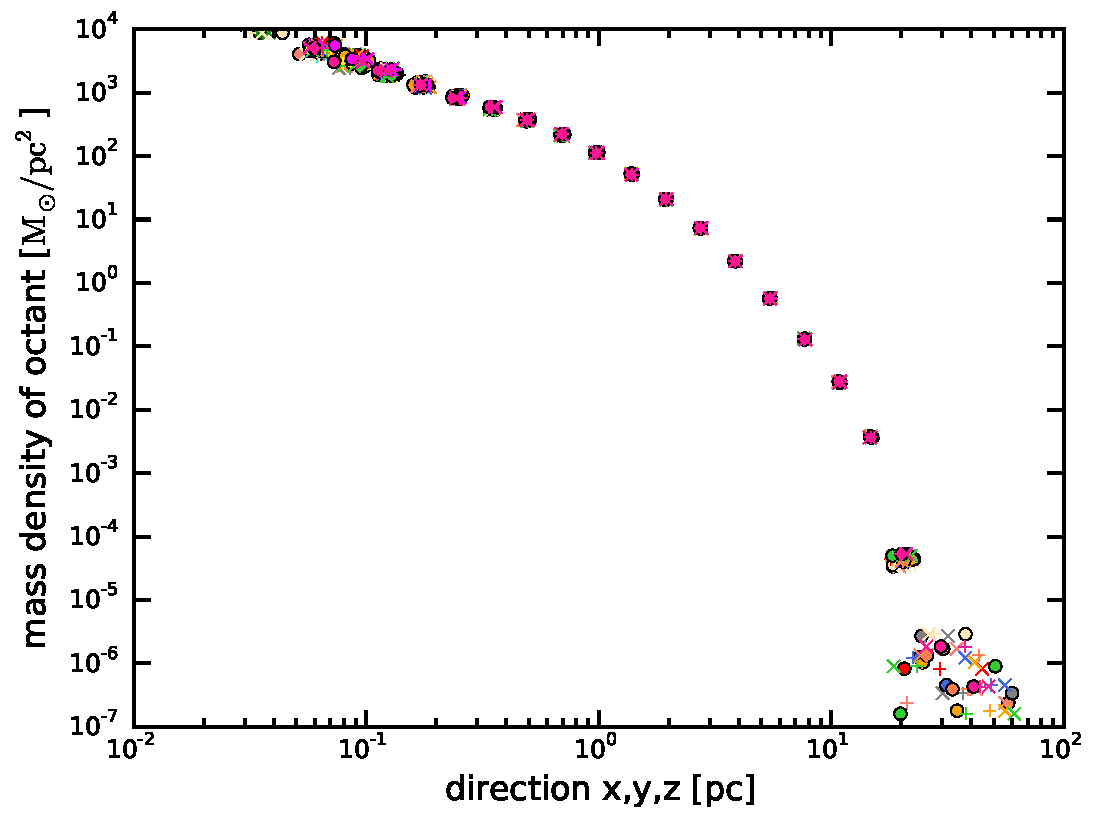
\includegraphics[width=0.7\textwidth]{Plots/sphericity_com.pdf}
\caption{Test for sphericity and center of mass of SIM 1.}
\label{fig:sphericity_com}
\end{figure}

\par From the density profile we can compute the potential as described in \ref{dens_pot_theory}. It is composed by the potential given from the stars and if there is one the potential of the \ac{IMBH} expressed as Kepler potential.
\begin{figure}[htbp]
	\centering
	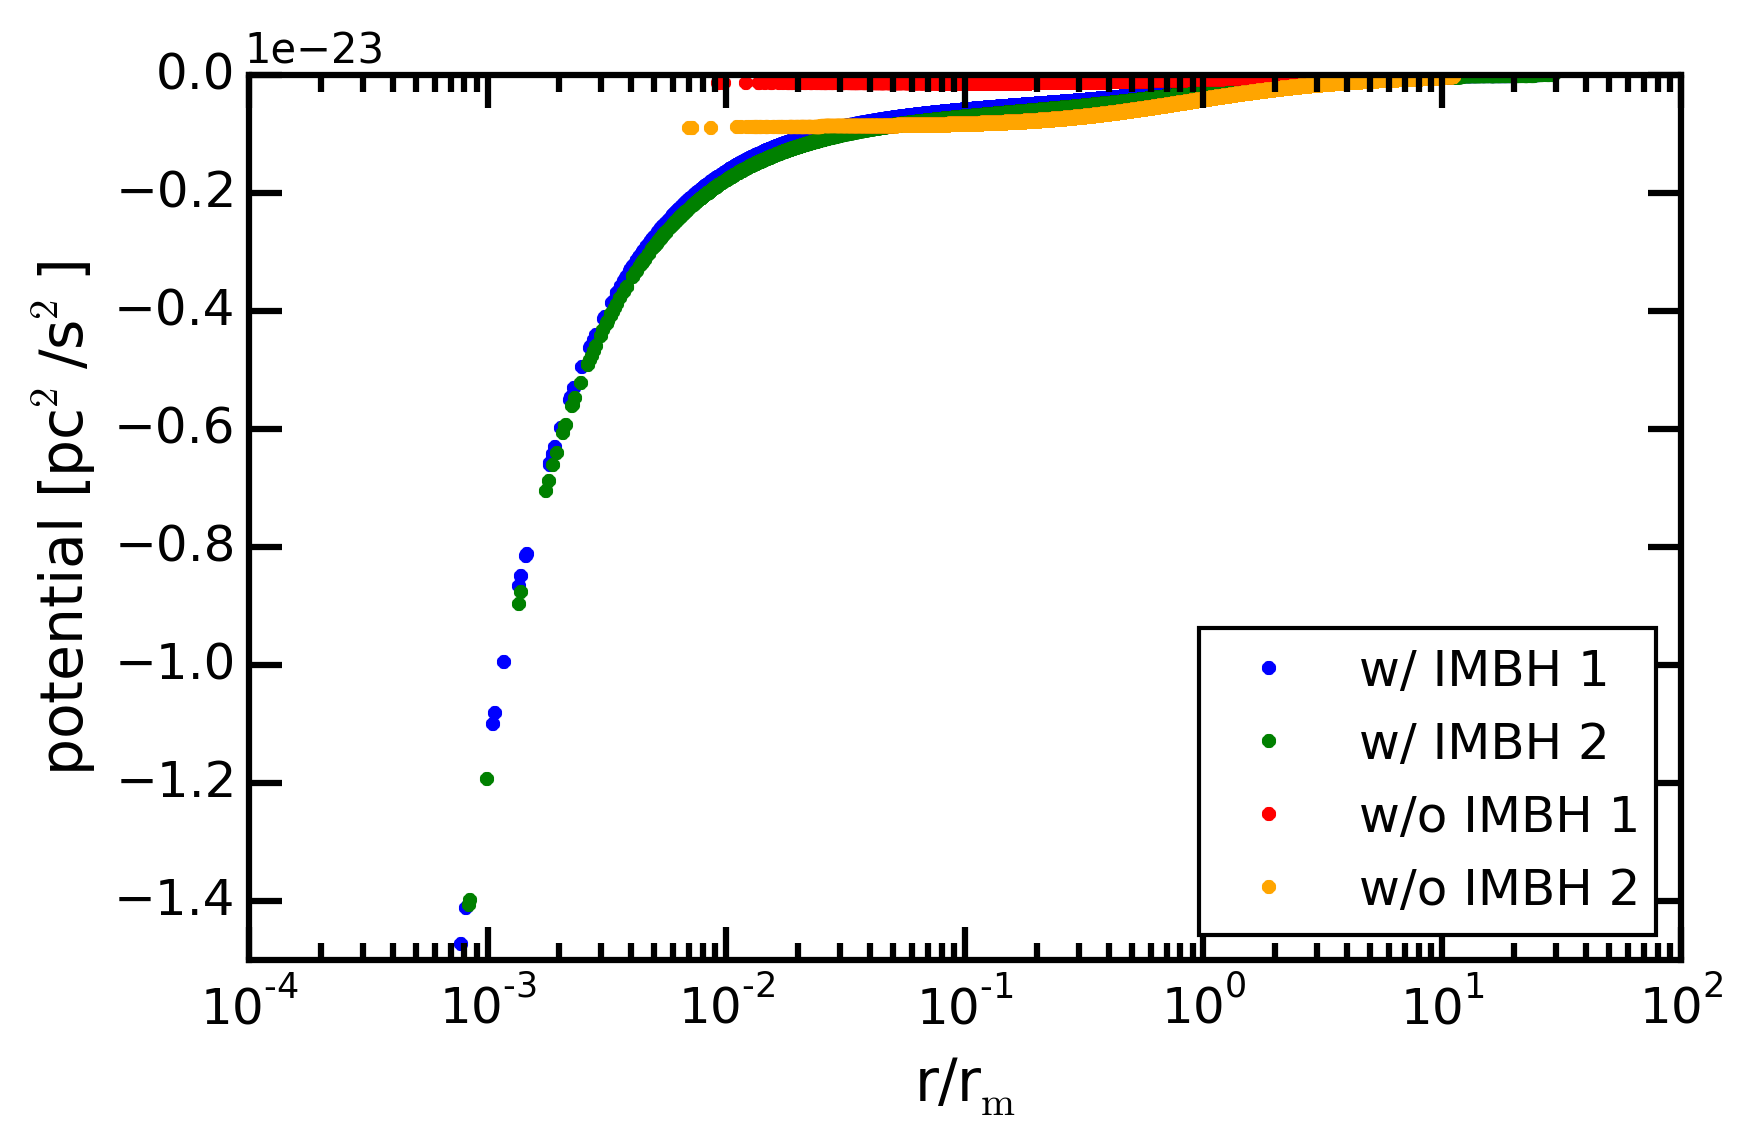
\includegraphics[width=0.475\textwidth]{Plots/potential.png}
	\caption{Potential of all \acp{GC}. SIM 1 and SIM 2 are nearly overlaying. They are the same simulation at different ages. The simulation lost 5 \% of its stars with 10 \% of the total mass while the \ac{IMBH} gained 13 \%. The potential of the stars declines while the potential of the \ac{IMBH} rises so the potential stays the same. The \acp{GC} without \ac{IMBH} remain constant in the inner part (until 0.5 half mass radii) and decrease from the points where their densities decrease.}
\end{figure}


\subsection{Investigations of orbits in action space}
\subsubsection{Orbits \& actions}


\subsubsection{Integral of motions along orbits}
